\chapterhead{2}{Where a Rolling Ball Goes}{Following the energy until the ball stops}\label{ch2}

A ball at the top of a ramp has stored energy. Let go, and the stored energy turns into \textbf{motion}. The ball rolls onto the floor and keeps going, but not forever. It slows and stops. Where did its motion go?

The floor and the ball rub against each other all the way. Rubbing turns motion into \textbf{warmth}, a tiny bit at every point. The warmth is too small to feel, so we follow the energy by what we can measure: the height at the start and the distance rolled.

\begin{center}
\sffamily\small\renewcommand{\arraystretch}{1.5}
\begin{tabular}{@{}p{3.4cm}p{3.7cm}p{3.7cm}@{}}
\toprule
\textbf{Model} & \textbf{What it keeps} & \textbf{What it drops}\\
\midrule
A ramp height & the stored energy at the start & the ball's spin\\
A roll distance & how far the motion lasted & the speed at each point\\
A surface & how much it rubs & its exact roughness\\
\bottomrule
\end{tabular}
\end{center}

\begin{tryit}{Roll it out}
\textbf{You need:} a board, books for a ramp 20~cm high, a ball, a tape measure, a bare floor, a rug and a towel.
\begin{enumerate}[leftmargin=1.6em]
\item Prop the board on books so its top end is 20~cm above the floor.
\item Release the ball from the top without pushing. Measure from the bottom of the ramp to where the ball stops.
\item Do three runs on each surface and average them.
\end{enumerate}
\par\medskip
\renewcommand{\arraystretch}{1.6}
\begin{tabular}{|l|c|c|c|c|}
\hline
\textbf{Surface} & \textbf{Run 1} & \textbf{Run 2} & \textbf{Run 3} & \textbf{Average (cm)}\\ \hline
Bare floor & & & & \\ \hline
Rug & & & & \\ \hline
Towel & & & & \\ \hline
\end{tabular}
\end{tryit}
\adult{Keep the ramp low and well away from stairs, and put the books where nobody will trip on them. Wipe any dust from the board first.}

\begin{worked}{Practice numbers, not from a real test}
Floor: 148, 152, 150, average 150~cm. Rug: 58, 52, 55, average 55~cm. Towel: 26, 24, 25, average 25~cm.\\
The same ball started with the same 20 units. On the towel it stopped after 25~cm, on the floor after 150~cm. A rougher surface rubs more, so the motion is used up sooner.
\end{worked}

\begin{center}
\begin{tikzpicture}
  \node[bigcir,minimum size=2.2cm] (a) at (0,0) {}; \node[font=\sffamily\scriptsize,align=center] at (0,0) {height\\20};
  \node[cir] (b) at (3.6,0) {20}; \node[cir] (c) at (7.2,0) {0};
  \node[font=\sffamily\scriptsize] at (3.6,-0.95) {motion}; \node[font=\sffamily\scriptsize] at (7.2,-0.95) {stopped};
  \draw[popA] (a) -- node[above,note] {roll starts} (b);
  \draw[moveA] (b) -- node[above,note] {rubbing} (c);
  \node[note,text width=3cm,align=center] at (5.4,-1.7) {The 20 did not vanish. It became warmth in the floor and ball.};
\end{tikzpicture}
\end{center}

\begin{multix}[hmm]\multixbot[hmm]\tcblower
The ball stopped, so its motion is gone. Zero left, nothing to find. I even drew a zero in the circle. Is that all?
\end{multix}

\trust{We used the same ball and the same ramp height for every surface, and did three runs on each.}
{The three runs on each surface were close together, so the average is steady. The towel always stopped it sooner than the rug.}
{How much warmth the ball made, because it is too small to feel. We name it, but we did not measure it.}

\begin{keepbox}
We turned a roll into one distance. \textbf{We kept} \wline[3.4cm] \textbf{and we set aside} \wline[3.4cm].
\end{keepbox}

\begin{tryit}{Higher ramp}
Use the bare floor. Set the ramp at 10~cm, 20~cm and 30~cm. Take three runs at each height and average them.\par\medskip
\renewcommand{\arraystretch}{1.6}
\begin{tabular}{|l|c|c|}
\hline
\textbf{Ramp height (units)} & \textbf{Average roll (cm)} & \textbf{Roll $\div$ height}\\ \hline
10 & & \\ \hline
20 & & \\ \hline
30 & & \\ \hline
\end{tabular}
\end{tryit}

\begin{worked}{Practice numbers}
Ramp 10: roll 75~cm. Ramp 20: roll 150~cm. Ramp 30: roll 225~cm.\\
$75\div10=7.5$, $150\div20=7.5$ and $225\div30=7.5$. Each unit of lift gave about 7.5~cm of roll on this floor.
\end{worked}

\begin{puzzle}{Average}
Three runs on a rug were 62, 58 and 60. Average \wline[1.6cm]~cm
\end{puzzle}

\begin{puzzle}{Which stops first?}
Floor 150, rug 55, towel 25. Which stops the ball soonest? \wline[2cm] How much shorter than the floor? \wline[1.6cm]~cm
\end{puzzle}

\begin{puzzle}{Unfair test}
Ana rolled a ball from a 10~cm ramp onto the rug. Ben used a 20~cm ramp on the floor. They say the floor is slippery. What is wrong? \wline[6cm]
\end{puzzle}

\begin{puzzle}{Predict}
On this floor each unit of lift gives 7.5~cm of roll. Predict the roll from a 40~cm ramp. \wline[1.6cm]~cm
\end{puzzle}

\begin{puzzle}{Fill the account}
A ball starts with 20 units of lift. After it stops, motion is \wline[1.6cm] and warmth gained is \wline[1.6cm].
\end{puzzle}

\clearpage

\begin{puzzle}{Which circle?}
Write S, M or W for stored, motion or warmth.\\
(a) ball at the top \wline[1cm] \quad (b) rolling on the floor \wline[1cm] \quad (c) stopped on the rug \wline[1cm]
\end{puzzle}

\begin{puzzle}{Why sooner?}
Why does a ball stop sooner on a rug than on a bare floor? \wline[6cm]
\end{puzzle}

\begin{puzzle}{Draw the circles}
Draw the ball on the floor as circles: height 20, then motion, then warmth.
\begin{center}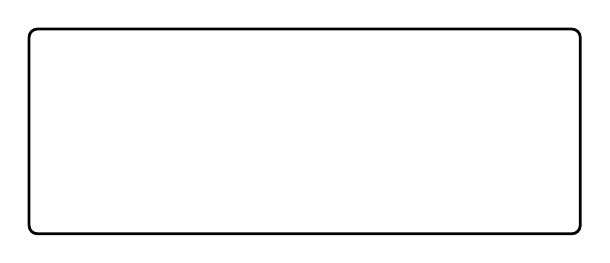
\begin{tikzpicture}\draw[line width=1pt,rounded corners=3pt] (0,0) rectangle (7,2.6); \end{tikzpicture}\end{center}
\end{puzzle}

\begin{puzzle}{Wrap}
A student wrote ``The rug destroyed the ball's motion.'' Wrap it with a better claim. \wline[6cm]
\end{puzzle}

\begin{puzzle}{Design a longer roll}
Say two changes that should make a ball roll farther, and one thing you would keep the same. \wline[6cm]
\end{puzzle}
\clearpage

\thispagestyle{fancy}
\subhead{Roll record}
Test three balls or three surfaces. Keep the ramp the same each time.\par\medskip
\renewcommand{\arraystretch}{3.0}
\begin{tabularx}{\linewidth}{|>{\sffamily\small\bfseries}p{2.6cm}|X|X|X|X|}
\hline
Ball and surface & Run 1 & Run 2 & Run 3 & Average \\ \hline
 & & & & \\ \hline
 & & & & \\ \hline
 & & & & \\ \hline
\end{tabularx}

\vspace{8pt}
Which rolled farthest? \wline[7cm]\\[10pt]
Which stopped soonest, and what might explain it? \wline[5cm]\\[10pt]
Sketch your ramp and mark where each ball stopped.\par\medskip
\begin{tikzpicture}\draw[ink!70,line width=1pt,rounded corners=3pt] (0,0) rectangle (11.4,5.2);\end{tikzpicture}
\clearpage
